\documentclass[border=1pt]{standalone}
% Shared preamble of the standalone figure sources (compiled to ../fig_*.pdf by build.sh).
\renewcommand{\rmdefault}{ptm}
\usepackage{amsmath,amssymb}
\usepackage[dvipsnames]{xcolor}
\usepackage{tikz}
\usetikzlibrary{arrows.meta,positioning,fit,calc,shapes.geometric,patterns,decorations.pathreplacing,backgrounds}
\usepackage{pgfplots}
\pgfplotsset{compat=1.17}
% ---------------------------------------------------------------------------
% Notation and helper macros (single source for symbols used in the paper)
% ---------------------------------------------------------------------------

% Placeholder for content that waits for the formal results or author input.
\newcommand{\todo}[1]{{\color{red}[\textbf{TODO:} #1]}}

% Generic
\newcommand{\R}{\mathbb{R}}
\newcommand{\SE}{\mathrm{SE}(3)}
\newcommand{\SO}{\mathrm{SO}(3)}
\newcommand{\T}{\top}
\newcommand{\E}{\mathbb{E}}
\newcommand{\norm}[1]{\left\lVert #1 \right\rVert}
\newcommand{\clip}{\operatorname{clip}}
\newcommand{\diag}{\operatorname{diag}}
\newcommand{\argmin}{\operatorname*{arg\,min}}
\newcommand{\lexmin}{\operatorname*{lex\,min}}

% Frames
\newcommand{\FI}{\mathcal{F}_{I}}
\newcommand{\FT}{\mathcal{F}_{T}}
\newcommand{\FC}{\mathcal{F}_{C}}
\newcommand{\FL}{\mathcal{F}_{L}}

% Mission
\newcommand{\Td}{T_{d}}            % mission deadline
\newcommand{\Dd}{\Delta_{d}}       % terminal reserve
\newcommand{\Lt}{L}                % latest admissible entry time
\newcommand{\Bmax}{B_{\max}}       % Delta-v budget
\newcommand{\dvused}{\Delta v_{\mathrm{u}}} % Delta-v used so far

% Geometry
\newcommand{\shat}{\hat{s}}
\newcommand{\er}{e_{r}}
\newcommand{\epol}{e_{\mathrm{pol}}}
\newcommand{\eaz}{e_{\mathrm{az}}}
\newcommand{\dlat}{\Delta\lambda}
\newcommand{\thg}{\theta_{g}}
\newcommand{\Tset}{\mathcal{T}}          % entry arrival-time candidates
\newcommand{\Wgeo}{\mathcal{W}_{\mathrm{geo}}}
\newcommand{\vb}{v_{b}}                  % braking envelope

% Decision and execution
\newcommand{\Bgrid}{\mathfrak{B}}        % candidate intent grid
\newcommand{\Bc}{\mathfrak{B}_{c}}       % certifiable candidate set
\newcommand{\Cmap}{\mathcal{C}}          % certification map
\newcommand{\zE}{z_{E}}                  % execution feedback
\newcommand{\PE}{P_{\mathcal{E}}}        % execution-layer macro kernel
\newcommand{\PC}{P_{\mathcal{C}}}        % certification-induced kernel
\newcommand{\gd}{\gamma_{d}}             % per-decision discount
\newcommand{\Hp}{H_{p}}                  % mode-prediction horizon
\newcommand{\ehat}{\hat{e}}
\newcommand{\tauhat}{\hat{\tau}}
\newcommand{\dvhat}{\widehat{\Delta v}}
\newcommand{\rtil}{\tilde{r}}

% Method names (fixed terminology, see fact sheet 00)
\newcommand{\ECC}{ECC}
\newcommand{\RWG}{RWG}

% Channel colors used in all method figures
\colorlet{actcol}{orange!85!black}   % action-level channel (screening)
\colorlet{actfill}{orange!14}
\colorlet{stcol}{blue!70!black}      % state-level channel (execution feedback)
\colorlet{stfill}{blue!7}
\colorlet{exefill}{green!8}
% Results figures: methods and outcomes, Okabe--Ito palette
\usepgfplotslibrary{fillbetween}
\definecolor{cECC}{HTML}{D55E00}    % ECC
\definecolor{cNOIN}{HTML}{E69F00}   % ECC w/o execution inputs (critic on the policy view)
\definecolor{cNOLE}{HTML}{0072B2}   % ECC w/o long-range entry (keep / correct only)
\definecolor{cNOCO}{HTML}{56B4E9}   % ECC w/o coordination
\definecolor{cSAC}{HTML}{555555}    % SAC--MPC
\definecolor{cTD3}{HTML}{000000}    % TD3--MPC
\definecolor{oCap}{HTML}{009E73}
\definecolor{oTime}{HTML}{BBBBBB}
\definecolor{oFuel}{HTML}{56B4E9}
\definecolor{oUns}{HTML}{CC79A7}
\pgfplotsset{resstyle/.style={tick label style={font=\scriptsize},label style={font=\footnotesize},
  legend style={font=\scriptsize,draw=none,fill=none},grid=major,grid style={gray!15},axis line style={gray!70!black}}}
% \band{group key}{color}{low column}{high column}: min--max band over seeds
\newcommand{\band}[4]{%
  \addplot[name path=lo#1#3,draw=none,forget plot] table[x=x,y=#3]{data/train_#1.dat};
  \addplot[name path=hi#1#3,draw=none,forget plot] table[x=x,y=#4]{data/train_#1.dat};
  \addplot[#2,fill opacity=0.15,forget plot] fill between[of=lo#1#3 and hi#1#3];}
% Case figures: execution modes (Table II)
\definecolor{cStage}{HTML}{0072B2}
\definecolor{cEntry}{HTML}{E69F00}
\definecolor{cHold}{HTML}{999999}
\definecolor{cDesc}{HTML}{009E73}
\colorlet{mStage}{cStage}\colorlet{mEntry}{cEntry}\colorlet{mHold}{cHold}\colorlet{mDesc}{cDesc}
% \modeband{t0}{t1}{mode style}: shaded mode interval over the full height of a time-history axis
\newcommand{\modeband}[3]{\fill[#3,opacity=0.13] ({axis cs:#1,1}|-{rel axis cs:0,0}) rectangle ({axis cs:#2,1}|-{rel axis cs:0,1});}

\begin{document}
% Kernels learned and executed: screening in training and execution (ECC) versus at execution only.
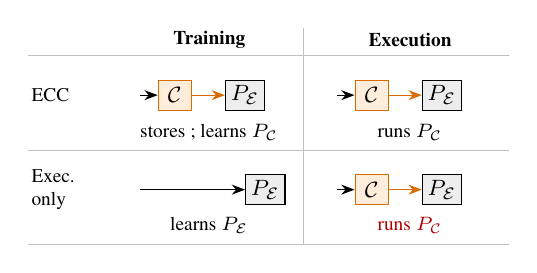
\begin{tikzpicture}[>=Stealth,font=\footnotesize,
  cb/.style={draw=actcol,fill=actfill,inner sep=1.5pt,minimum width=0.42cm,minimum height=0.38cm},
  pb/.style={draw,fill=gray!14,inner sep=1.5pt,minimum width=0.5cm,minimum height=0.38cm},
  hd/.style={font=\scriptsize\bfseries,inner sep=1pt},
  rl/.style={font=\scriptsize,align=left,anchor=west,inner sep=1pt}]
  \node[hd] at (1.55,1.15) {Training};
  \node[hd] at (4.1,1.15) {Execution};
  \draw[gray!50] (-0.75,0.95) -- (5.35,0.95);
  \node[rl] at (-0.75,0.45) {ECC};
  \node (a1) at (0.55,0.45) {$\ba$}; \node[cb,right=0.22cm of a1] (c1) {$\Cmap$}; \node[pb,right=0.42cm of c1] (p1) {$\PE$};
  \draw[->] (a1) -- (c1); \draw[->,actcol] (c1) -- node[above,font=\scriptsize,inner sep=1pt] {$\atil$} (p1);
  \node (a2) at (3.05,0.45) {$\ba$}; \node[cb,right=0.22cm of a2] (c2) {$\Cmap$}; \node[pb,right=0.42cm of c2] (p2) {$\PE$};
  \draw[->] (a2) -- (c2); \draw[->,actcol] (c2) -- node[above,font=\scriptsize,inner sep=1pt] {$\atil$} (p2);
  \node[font=\scriptsize,inner sep=1pt,align=center] at (1.55,-0.02) {stores $\ba$; learns $\PC$};
  \node[font=\scriptsize,inner sep=1pt] at (4.1,-0.02) {runs $\PC$};
  \draw[gray!50] (-0.75,-0.25) -- (5.35,-0.25);
  \node[rl,align=left] at (-0.75,-0.75) {Exec.\\only};
  \node (a3) at (0.55,-0.75) {$\ba$}; \node[pb,right=1.33cm of a3] (p3) {$\PE$};
  \draw[->] (a3) -- (p3);
  \node (a4) at (3.05,-0.75) {$\ba$}; \node[cb,right=0.22cm of a4] (c4) {$\Cmap$}; \node[pb,right=0.42cm of c4] (p4) {$\PE$};
  \draw[->] (a4) -- (c4); \draw[->,actcol] (c4) -- node[above,font=\scriptsize,inner sep=1pt] {$\atil$} (p4);
  \node[font=\scriptsize,inner sep=1pt] at (1.55,-1.2) {learns $\PE$};
  \node[font=\scriptsize,red!70!black,inner sep=1pt] at (4.1,-1.2) {runs $\PC$};
  \draw[gray!50] (-0.75,-1.45) -- (5.35,-1.45);
  \draw[gray!50] (2.75,1.3) -- (2.75,-1.45);
\end{tikzpicture}
\end{document}
